% Appendix A

\chapter{Appendix Title Here} % Main appendix title

\label{AppendixA} % For referencing this appendix elsewhere, use \ref{AppendixA}

\lhead{Appendix A. \emph{Appendix Title Here}} % This is for the header on each page - perhaps a shortened title

\section{Crawlers XML Configuration File}
\label{crawlersXML}
\lstset{ %
  language=XML,                % the language of the code
  basicstyle=\footnotesize,           % the size of the fonts that are used for the code
  numbers=left,                   % where to put the line-numbers
  numberstyle=\tiny\color{gray},  % the style that is used for the line-numbers
  stepnumber=2,                   % the step between two line-numbers. If it's 1, each line 
                                  % will be numbered
  numbersep=5pt,                  % how far the line-numbers are from the code
  backgroundcolor=\color{white},      % choose the background color. You must add \usepackage{color}
  showspaces=false,               % show spaces adding particular underscores
  showstringspaces=false,         % underline spaces within strings
  showtabs=false,                 % show tabs within strings adding particular underscores
  frame=single,                   % adds a frame around the code
  rulecolor=\color{black},        % if not set, the frame-color may be changed on line-breaks within not-black text (e.g. commens (green here))
  tabsize=2,                      % sets default tabsize to 2 spaces
  captionpos=b,                   % sets the caption-position to bottom
  breaklines=true,                % sets automatic line breaking
  breakatwhitespace=false,        % sets if automatic breaks should only happen at whitespace
  title=\lstname,                   % show the filename of files included with \lstinputlisting;
                                  % also try caption instead of title
  keywordstyle=\color{blue},          % keyword style
  commentstyle=\color{dkgreen},       % comment style
  stringstyle=\color{mauve},         % string literal style
  escapeinside={\%*}{*)},            % if you want to add a comment within your code
  morekeywords={*,...}               % if you want to add more keywords to the set
}
\begin{lstlisting}
<?xml version="1.0" encoding="UTF-8"?>

<config charset="UTF-8">

    <!-- set initial page -->
    <var-def name="home">http://ara.reuters.com/</var-def>

    <!-- define script functions and variables -->
    <script><![CDATA[
        /* checks if specified URL is valid for download */
        boolean isValidUrl(String url) {
            String urlSmall = url.toLowerCase();
            return (urlSmall.startsWith("http://ara.reuters.com/")&& !urlSmall.contains(" ")&& !urlSmall.contains("javascript"));
        }

        /* create filename based on specified URL */
        String makeFilename(String url) {
        	String temp = url.replaceAll("http://|https://|file://", "");
        	temp = temp.replaceAll("\\s","");
        	temp = temp.replaceAll("\\:","");
           	return temp.replaceAll("\\?","");
        }
		String makeFile(String url) {
		String temp = "http://ara.reuters.com";
		if(url!= null&&!url.toLowerCase().contains("javascript")&&url.startsWith("http://ara.reuters.com/")){
			temp = url.replaceAll("http://|https://|file://", "");
			temp = temp.replaceAll("\\:","");
	        temp = temp.replaceAll("\\s","");
		}
	        return temp;
        }
        /* set of unvisited URLs */
        Set unvisited = new HashSet();
        unvisited.add(home);

        /* pushes to web-harvest context initial set of unvisited pages */
        SetContextVar("unvisitedVar", unvisited);

        /* set of visited URLs */
        Set visited = new HashSet();
    ]]></script>

    <!-- loop while there are any unvisited links -->
    <while condition="${unvisitedVar.toList().size() != 0}">
        <loop item="currUrl">
            <list><var name="unvisitedVar"/></list>
            <body>
                <empty>
                    <var-def name="content">
                        <html-to-xml>
                            <http url="${currUrl}"/>
                         </html-to-xml>
                    </var-def>

                    <script><![CDATA[
                        currentFullUrl = sys.fullUrl(home, currUrl);
                    ]]></script>

                    <!--  saves downloaded page -->
                    <file action="write" path="spider/${makeFilename(currentFullUrl)}.html">
                        <var name="content"/>
                    </file>
	                    

                    <!-- adds current URL to the list of visited -->
                    <script><![CDATA[
                        visited.add(sys.fullUrl(home, currUrl));
                        Set newLinks = new HashSet();
                        print(currUrl);
                    ]]></script>

                    <!-- loop through all collected links on the downloaded page -->
                    <loop item="currLink">
                        <list>
                            <xpath expression="//a/@href">
                                <var name="content"/>
                            </xpath>
                        </list>
                        <body>
                            <script><![CDATA[
                                String fullLink = sys.fullUrl(home, currLink);
                                if ( isValidUrl(fullLink.toString()) && !visited.contains(fullLink) && !unvisitedVar.toList().contains(fullLink) ) {
                                    newLinks.add(fullLink);
                                }
                            ]]></script>
                            
                            <file action="write" path="spiders/reuters/reuters${makeFilename(sys.fullUrl(home, currLink))}.txt" charset="UTF-8">
                            <xquery>
	                            <xq-param name="doc">
	                        		<html-to-xml>
					                   <try>
				        					<body>
	                          		  			<http url="${makeFile(sys.fullUrl(home, currLink))}"/>
	                          		  			</body>
									        <catch>
									            No report file!
									        </catch>
									    </try>
	                        		</html-to-xml>
	                    		</xq-param>
			                      <xq-expression><![CDATA[
			                      declare variable $doc as node() external;
                  			      let $title := data($doc//title)
                  			      let $text := data($doc//div[@id="resizeableText"])
			                            return
			                                <article>
			                                    <title>{data($title)}</title>
								    			<text>{data($text)}</text>
    			                                </article>
			                    ]]></xq-expression>
			                </xquery>
			                
			                <![CDATA[ </reuters/reuters> ]]>
			                </file>
                        </body>
                    </loop>
                </empty>
            </body>
        </loop>

        <!-- unvisited link are now all the collected new links from downloaded pages  -->
        <script><![CDATA[
             SetContextVar("unvisitedVar", newLinks);
        ]]></script>
    </while>

</config>
\end{lstlisting}

\section{JIGSAW Disambiguation}
\label{jigsaw}
\begin{figure}[htbp]
	\centering
		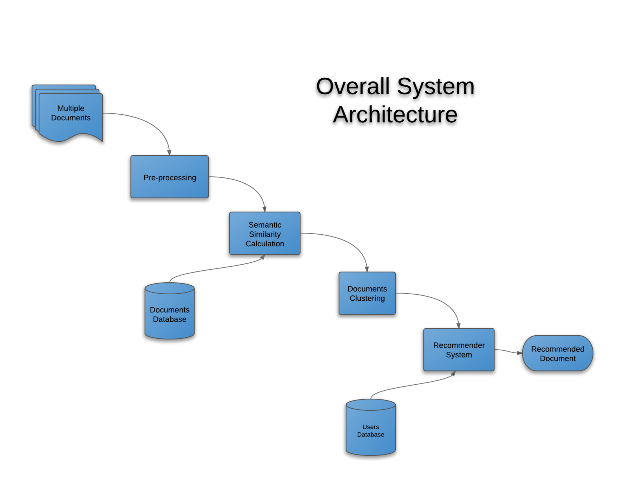
\includegraphics{./Figures/System Architecture.png}
		\rule{35em}{0.0001pt}
	\caption[Web-Harvest}
\end{figure}
